\begin{figure}[h] 
\centering 
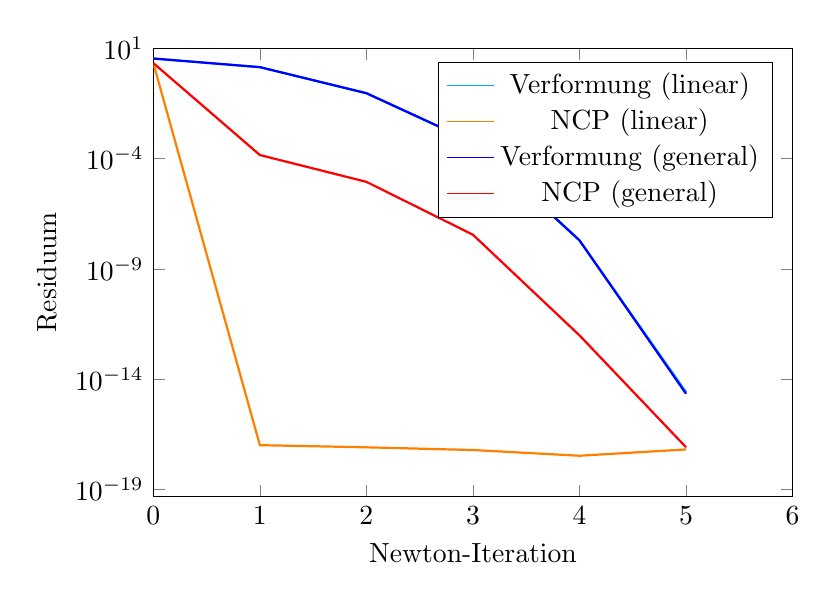
\begin{tikzpicture}[every plot/.append style={thick}] 
\begin{axis}[ 
label style={font=\normalsize}, 
xlabel={Newton-Iteration}, 
ylabel={Residuum}, 
xmin=0, xmax=6, 
ymode=log, 
ymin=0, ymax=10, 
width=0.8\textwidth, 
height=0.6\textwidth, 
legend pos=north east, 
legend style={cells={align=left}}, 
grid style=dashed, 
] 
\addplot[ 
color=cyan, 
] 
coordinates { 
(0, 3.39e+00)(1, 1.38e+00)(2, 9.09e-02)(3, 5.45e-04)(4, 1.93e-08)(5, 2.61e-15)}; 
\addlegendentry{Verformung (linear)} 
\addplot[ 
color=orange, 
] 
coordinates { 
(0, 2.11e+00)(1, 1.03e-17)(2, 8.24e-18)(3, 6.20e-18)(4, 3.42e-18)(5, 6.59e-18)}; 
\addlegendentry{NCP (linear)} 
\addplot[ 
color=blue, 
] 
coordinates { 
(0, 3.39e+00)(1, 1.38e+00)(2, 9.11e-02)(3, 5.51e-04)(4, 1.97e-08)(5, 2.19e-15)}; 
\addlegendentry{Verformung (general)} 
\addplot[ 
color=red, 
] 
coordinates { 
(0, 2.11e+00)(1, 1.44e-04)(2, 8.77e-06)(3, 3.52e-08)(4, 9.70e-13)(5, 8.30e-18)}; 
\addlegendentry{NCP (general)} 
\end{axis} 
\end{tikzpicture} 
\caption{Residuen des Stoffgesetzes 'St.Venant' mit Hinderniss 'Parabel' und 50 Freiheitsgraden für die Verschiebung.} 
\label{fiq:St.Venant_Parabel_level1} 
\end{figure} 
